\documentclass[]{elsarticle} %review=doublespace preprint=single 5p=2 column
%%% Begin My package additions %%%%%%%%%%%%%%%%%%%

\usepackage[hyphens]{url}


\usepackage{graphicx}
%%%%%%%%%%%%%%%% end my additions to header

\usepackage[T1]{fontenc}
\usepackage{lmodern}
\usepackage{amssymb,amsmath}
% TODO: Currently lineno needs to be loaded after amsmath because of conflict
% https://github.com/latex-lineno/lineno/issues/5
\usepackage{lineno} % add
\usepackage{ifxetex,ifluatex}
\usepackage{fixltx2e} % provides \textsubscript
% use upquote if available, for straight quotes in verbatim environments
\IfFileExists{upquote.sty}{\usepackage{upquote}}{}
\ifnum 0\ifxetex 1\fi\ifluatex 1\fi=0 % if pdftex
  \usepackage[utf8]{inputenc}
\else % if luatex or xelatex
  \usepackage{fontspec}
  \ifxetex
    \usepackage{xltxtra,xunicode}
  \fi
  \defaultfontfeatures{Mapping=tex-text,Scale=MatchLowercase}
  \newcommand{\euro}{€}
\fi
% use microtype if available
\IfFileExists{microtype.sty}{\usepackage{microtype}}{}
\usepackage[]{natbib}
\bibliographystyle{plainnat}

\usepackage{graphicx}
\ifxetex
  \usepackage[setpagesize=false, % page size defined by xetex
              unicode=false, % unicode breaks when used with xetex
              xetex]{hyperref}
\else
  \usepackage[unicode=true]{hyperref}
\fi
\hypersetup{breaklinks=true,
            bookmarks=true,
            pdfauthor={},
            pdftitle={A Density-Based approach to identify Home location for College Communities from Big Data},
            colorlinks=false,
            urlcolor=blue,
            linkcolor=magenta,
            pdfborder={0 0 0}}

\setcounter{secnumdepth}{5}
% Pandoc toggle for numbering sections (defaults to be off)


% tightlist command for lists without linebreak
\providecommand{\tightlist}{%
  \setlength{\itemsep}{0pt}\setlength{\parskip}{0pt}}

% From pandoc table feature
\usepackage{longtable,booktabs,array}
\usepackage{calc} % for calculating minipage widths
% Correct order of tables after \paragraph or \subparagraph
\usepackage{etoolbox}
\makeatletter
\patchcmd\longtable{\par}{\if@noskipsec\mbox{}\fi\par}{}{}
\makeatother
% Allow footnotes in longtable head/foot
\IfFileExists{footnotehyper.sty}{\usepackage{footnotehyper}}{\usepackage{footnote}}
\makesavenoteenv{longtable}






\begin{document}


\begin{frontmatter}

  \title{A Density-Based approach to identify Home location for College
Communities from Big Data}
    \author[1]{Iván Mendoza%
  \corref{cor1}%
  }
   \ead{imendoza@uazuay.edu.ec} 
    \author[1]{Andrés Baquero%
  %
  }
   \ead{obaquero@uazuay.edu.ec} 
    \author[1]{Gustavo Álvarez%
  %
  }
   \ead{galvarezc@uazuay.edu.ec} 
      \cortext[cor1]{Corresponding author}
  
  \begin{abstract}
  In the era of big data, the abundance of information presents
  unprecedented opportunities to gain valuable insights into human
  behavior and activities. This study focuses on harnessing the power of
  data collected from mobile applications used by students at a local
  college, with the aim of identifying the location of their homes. By
  filtering these locations, the study seeks to improve the
  understanding of mobility patterns and the most frequent points of
  interest among students, to obtain useful information for
  decision-making in mobility-related issues and transportation planning
  in the surrounding areas. In this paper, a density-based heuristic is
  proposed to detect home location from big data, which are collected in
  real-time by a mobile application. The results were satisfactory and
  their precision seems to increase as more data is acquired, which
  allows providing insights about potential future applications.
  \end{abstract}
    \begin{keyword}
    Big data \sep data mining \sep home detection \sep mobility
patterns \sep 
    points of interest
  \end{keyword}
  
 \end{frontmatter}

\hypertarget{introduction}{%
\section{Introduction}\label{introduction}}

Gaining insights into the mobility patterns and points of interest among
college students is crucial in developing effective strategies to
optimize transportation for both students and the entire city. In the
scope of this study, our objective is to identify and analyze the
precise locations of student residences from a college community,
utilizing mobile app data.

Mobile phone data can be a useful source for official statistics, but
there are challenges and uncertainties that need to be addressed before
they can be used. Detecting home locations from mobile phone data and
analyzes the performance of five home detection algorithms, offering
recommendations for more reliable use of mobile phone data in official
statistics.

Some studies like \citep{osorio2019social} demonstrates the potential of
using social media data, specifically Twitter, for studying urban
mobility patterns. However, the authors note the limitations of the
data, such as biases in social media usage and the need for ongoing
validation and improvement of the methods used. In other study
\citep{pappalardo2021evaluation} about Home Detection Algorithms (HDAs)
using mobile phone data for official statistics. The authors found that
the type of data stream used, and the algorithm choice significantly
influenced the accuracy of home detection. Algorithms based on weekdays
and/or nighttime records were the most accurate and using Extended
Detail Records (XDRs) with specific algorithms yielded the best results.
Daytime records and spatial perimeter-based algorithms had low accuracy
and should be avoided. XDRs and Cellular Positioning Records (CPRs) were
more resilient to data reduction compared to Call Detail Records (CDRs).
The study had limitations in sample size and lack of demographic
information. In \citep{ahas2010using} concludes that mobile positioning
data can be used to monitor population geography and mobility,
particularly in socially unstable or rapidly developing regions.
However, further work is needed to standardize the data and model for
different sources and conditions. The methodology is promising for
geographical research and offers opportunities for real-time monitoring
tools, geographical applications, tourism development, traffic
management, urban planning, and optimizing network services. Detecting
the location of households from mobile phone data is a key challenge for
the use of this data source in official statistics. The authors argue
that current address detection methods suffer from a lack of consensus
on criteria and limited validation capabilities. The article presents an
analysis of five address detection algorithms applied to a large French
Call Detail Record (CDR) dataset, showing that the choice of criteria in
Home Detection Algorithms (HDAs) influences address location detection
in up to 40\% of users, and that HDAs perform poorly when compared to a
validation dataset. In \citep{gauvin2020gender} the authors used mobile
phone data and metadata, including call detail records (CDRs) enriched
with gender, socioeconomic segment, and number of phone lines registered
under that number. then analyzed the data to reveal a gender gap in
mobility and mapped this mobility gap over administrative divisions to
observe the association with lower income and lack of public and private
transportation options. The paper concludes that there is a gender gap
in urban mobility, where women visit fewer unique locations than men and
distribute their time less equally among such locations. This mobility
gap is associated with lower income and lack of public and private
transportation options. In \citep{vanhoof2018assessing} the paper
investigates the performance and capabilities of five popular criteria
for home detection based on a very large mobile phone dataset from
France. The study shows that most Home Detection Algorithms (HDAs)
suffer from ``blind'' deployment of criteria to define homes and from
limited possibilities for validation. The paper introduces a data-driven
framework to assess the spatial uncertainty related to the application
of HDAs. The findings appropriate spatial uncertainty in HDA and, in
extension, for detection of meaningful places. The study shows how
spatial uncertainties on the individuals' level can be assessed in
absence of ground truth annotation, how they relate to traditional,
high-level validation practices and how they can be used to improve
results for, e.g., nation-wide population estimation. Therefore, the
paper concludes that the proposed framework can be used to improve the
accuracy of home detection algorithms and population estimation. In
\citep{bojic2015choosing} the authors discuss the importance of knowing
user location in the digital world, not only in real-time but also
predicting future locations. It is necessary to semantically label a
place, particularly detecting the most probable home location for a
given user. The paper aims to provide insights on the differences among
the ways how different types of human digital trails represent actual
mobility patterns and the differences between the approaches
interpreting those trails for inferring said patterns. The paper starts
with an example showing how human mobility patterns described by means
of radius of gyration are different for Flickr social network and
dataset of bank card transactions. The paper considers several methods
for home location definition known from the literature and demonstrates
that although for bank card transactions they provide highly consistent
results, home location definition detection methods applied to Flickr
dataset happen to be way more sensitive to the method selected,
stressing the paramount importance of adjusting the method to the
specific dataset being used.In universities, there is a need to enhance
student mobility, and various strategies have been suggested to achieve
this goal. To implement effective policies, it is crucial to have
dynamic origin-destination matrices (OD) that represent different
scenarios. The widespread use of mobile devices has made it possible to
automatically extract daily travel data through tracking apps,
eliminating the need for traditional trip surveys. Mendoza et. al
\citep{mendoza2020automatic} presents a new methodology for extracting
multi-day mobility demand in universities using logs obtained from
dedicated apps regularly used by students. The proposed approach was
evaluated using real-life logs from a representative group of students
over a five-month period. The results showed that this approach is
effective in obtaining average demand data, which can be utilized in
planning mobility strategies, as long as continuous tracking of mobility
data is feasible through mobile devices.

The primary objective of this study is to filter out student homes from
the collected mobile app data and categorize them. By accurately
identifying these locations, we can lay the foundation for a more
comprehensive analysis of student mobility patterns and points of
interest.

This research is part of a larger investigation focused on understanding
the unique needs and preferences of a college community. By identifying
their homes, we gain crucial insights into their daily commute patterns,
transportation modes, and the places they frequent. Such information
enables the college authorities and municipal stakeholders, to make
data-driven decisions and develop tailored mobility plans that cater to
the specific needs of the student population.

In this paper, we present the methodology used to collect and preprocess
the mobile app data, with a specific focus on identifying student homes.
We discuss the techniques employed to filter and categorize these
locations accurately. Additionally, we delve into the analysis of
student mobility patterns and points of interest derived from the
identified residences. The results and their implications for
decision-making are presented and discussed in detail. The findings from
this study will provide valuable to the understanding their mobility
patterns, decision-makers can develop targeted interventions, optimize
transportation systems, and create a supportive environment for the
student community. This research underscores the significance of
leveraging mobile app data to gain a comprehensive understanding of
student mobility patterns and points of interest, facilitating
evidence-based decision-making and the development of effective mobility
plans.

For this approach, a density-based heuristic is proposed to detect home
location from big data, which are collected in real-time by a dedicated
mobile application developed for this purpose. This document is
organized in the following way: a literature review of related works
about origin-destination (OD) and home detection; then a detailed
explanation of the methodology. At the end, conclusions, then a
discussion of results and future works are proposed to provide insights
about potential future applications and research.

\hypertarget{methodology}{%
\section{Methodology}\label{methodology}}

The Resulting locations of the student homes have to be mined from
mobility data after these are processed following a multi-step
procedure. The required steps are summarized through the flow chart
found in Figure \ref{fig1}, then a deeper explanation follows in the
next sections.

\begin{figure}
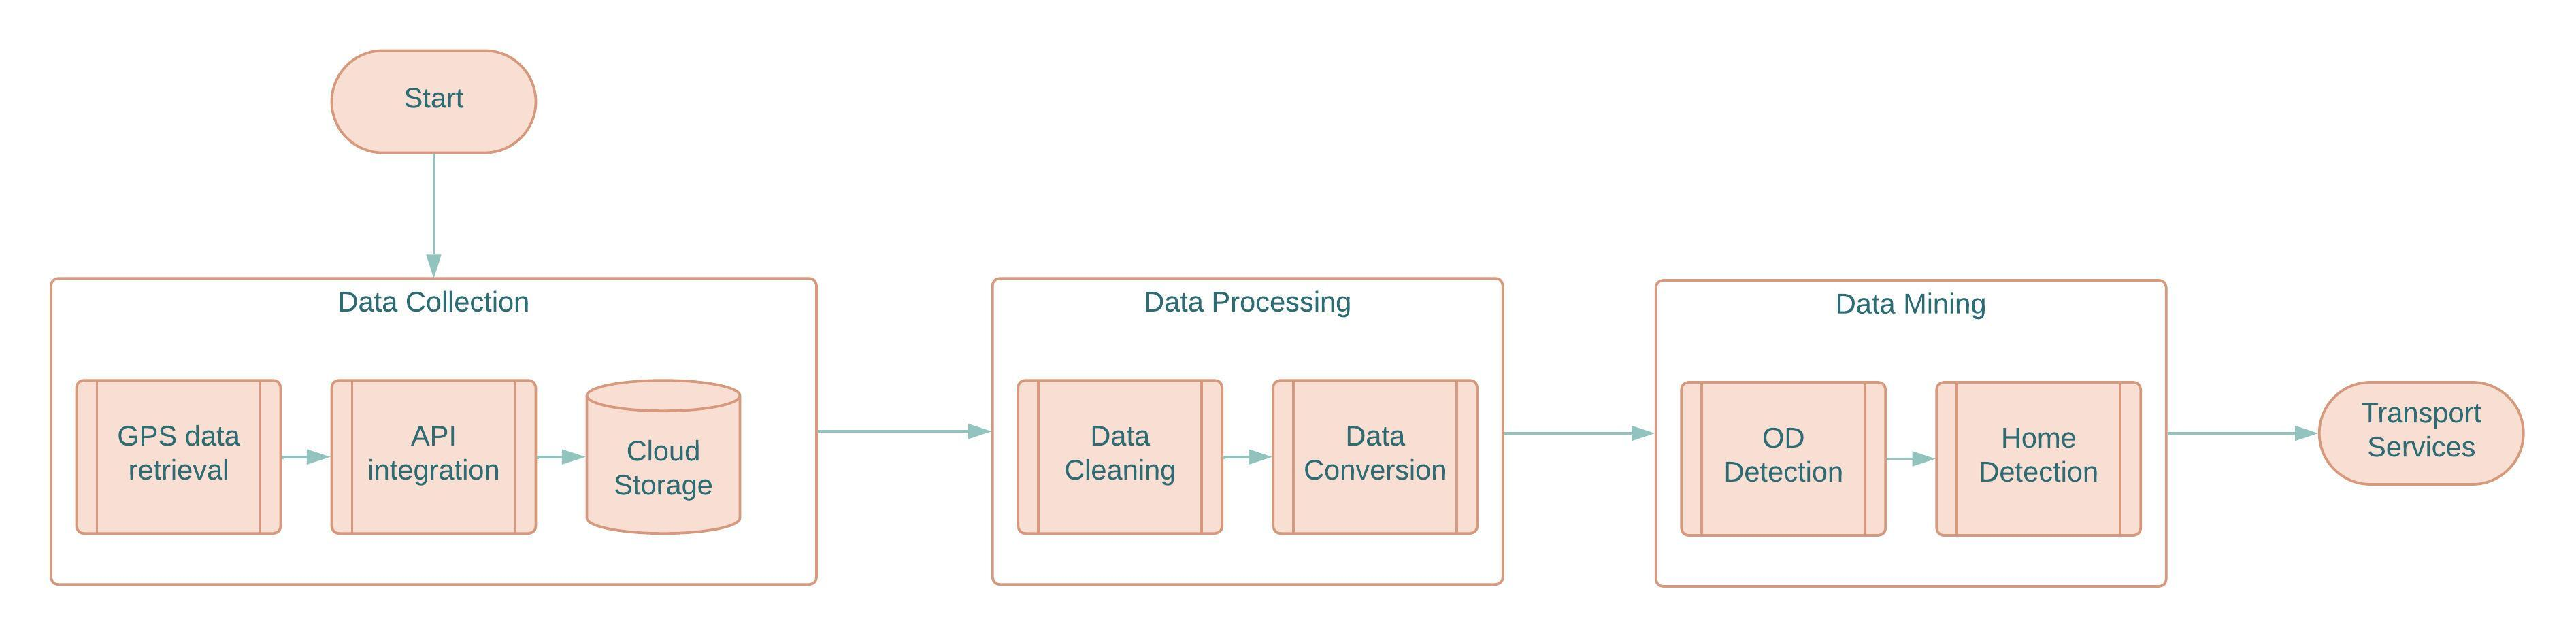
\includegraphics[width=0.9\linewidth]{../paper/images/Methodology Home Detection} \caption{\label{fig1}Multi-step procedure methodology for Big Data Home Detection.}\label{fig:unnamed-chunk-1}
\end{figure}

In a few words, data are collected by a mobile app which uses the Global
Positioning System (GPS) sensors of the mobile device, so that they can
be stored in a remote server via an Application Programming Interface
(API). Then, these unprocessed data are cleaned to filter out outliers
and transformed to a suitable format for further calculations. At last,
origins and destinations (OD) are detected by some segmentation
algorithm and later classified as potential home locations. Some
potential transport services after acquiring this information are
planned out to complete the flow.

\hypertarget{mobile-data-collection}{%
\subsection{Mobile Data Collection}\label{mobile-data-collection}}

The first step, assuming a mobile app exists so that it can collect GPS
data, is storing mobility data together with temporal and identity
information in a remote database. Each observation \emph{i} (a labeled
spatiotemporal data point) will have the following structure:

\[ p_i = (x_i, y_i, t_i) \] that is, in its simplest form, it consists
on the location's coordinates \((x,y)\) of the tracked user at a
specific time \emph{t}. A more complete version of the observation is:

\[ p_i  = (uid_i, lat_i, lon_i, alt_i, date_i, t_i, dow_i, acc_i, timestamp_i) \]

\begin{itemize}
\item
  \emph{uid}, is a user's unique identifier, normally a MD5 hash string
  which guarantees data is collected anonymously, but it still makes
  possible to know the user in the database.
\item
  \emph{lat. lon, alt}, the point's latitude, longitude and altitude
  coordinates.
\item
  \emph{date}, a day-month-year string
\item
  \emph{t}, a 24-hour local time format for a continuous variable after
  applying this formula:
\end{itemize}

\[ t  =  hours + \frac{minutes}{60} + \frac{seconds}{3600}\]

\begin{itemize}
\item
  \emph{dow}, the day of the week the observation was captured, where 1
  is Sunday
\item
  \emph{acc}, accuracy in meters of the measurement as reported by the
  sensor API, lower values produce more accurate measurements.
\item
  \emph{timestamp}, A Unix based time stamp, allowing to treat dates as
  continuous variables.
\end{itemize}

The set \(P_a\) of data point observations collected in real-time by a
user's mobile device, is stored in this format in a remote server for
further off-line procedures. However, this format is not yet suitable
for most calculations, so that further processing is required as
described in the next steps.

\hypertarget{data-processing}{%
\subsection{Data Processing}\label{data-processing}}

In order to avoid bias in the calculation of travel destinations,
outliers are removed considering position accuracy and temporal
constraints. A subset \(P_a\) consists of more refined ``valid''
observations, selected through the following criteria.

\[ P_b  =  \{p_i\in P_a | acc_i< \alpha \}\] where \(\alpha\) is a
parameter that denotes the maximum allowed accuracy error in meters.
Moreover, users can travel to destinations found in other regions,
countries and even continents. For the purpose of this research, home
locations must be found inside a study region at a medium-sized city
level, so a bounding box defined by
\([lon_{min}, lon_{max}, lat_{min}, lat_{max}]\) constraints the valid
observation previously found.

\[ P_c  =  \{p_i\in P_b | (lat_{min}<lat_i<lat_{max}) \wedge   (lon_{min}<lon_i<lon_{max}) \}\]
Because this research is intended to provide insights about transport
services for students in a College Community, a time period where users
are expected to regularly visit the campus must be selected. Then, a
cutoff date defined by \([date_{min}, date_{max}]\) is used to select
the final subset \(P\).

\[ P  =  \{p_i\in P_c | (date_{min}<date_i<date_{max}) \}\]

At last, since OD detection requires computation of distances, a
Cartesian projection is a better approach. For the selected study region
the UTM-17S is chosen, so that longitude, latitude and altitude measures
are transformed to euclidean space coordinates \((x,y,z)\). Since dates
and accuracies are not needed anymore, each observation \(p_i\) in the
resulting processed set \(P\) becomes:

\[ p_i  = (uid_i, x_i, y_i, z_i, t_i, dow_i) \]

\hypertarget{dataset-description}{%
\subsubsection{Dataset Description}\label{dataset-description}}

The full dataset used in this study consists of spatiotemporal data,
collected by a dedicated tracking mobile app for a College Community. It
involves data from \emph{728} users during one moth period, namely from
May 20 to June 20, 2023. The results of the further analysis have proven
30 days of mobility data per user to be sufficient to identify home
locations. The number of observations after the data cleaning process is
above \emph{11 million}, so that good infrastructure of the cloud
storage is required to handle this volume of big data.

A sample from the spatiotemporal dataset is presented below in Table
\ref{tab1} for the five attributes mentioned earlier:

\begin{longtable}[]{@{}
  >{\centering\arraybackslash}p{(\columnwidth - 12\tabcolsep) * \real{0.1818}}
  >{\centering\arraybackslash}p{(\columnwidth - 12\tabcolsep) * \real{0.1515}}
  >{\centering\arraybackslash}p{(\columnwidth - 12\tabcolsep) * \real{0.1364}}
  >{\centering\arraybackslash}p{(\columnwidth - 12\tabcolsep) * \real{0.1212}}
  >{\centering\arraybackslash}p{(\columnwidth - 12\tabcolsep) * \real{0.1515}}
  >{\centering\arraybackslash}p{(\columnwidth - 12\tabcolsep) * \real{0.0758}}
  >{\centering\arraybackslash}p{(\columnwidth - 12\tabcolsep) * \real{0.1818}}@{}}
\caption{\label{tab1}Sample observations from the Spatiotemporal
Dataset}\tabularnewline
\toprule()
\begin{minipage}[b]{\linewidth}\centering
uid
\end{minipage} & \begin{minipage}[b]{\linewidth}\centering
x
\end{minipage} & \begin{minipage}[b]{\linewidth}\centering
y
\end{minipage} & \begin{minipage}[b]{\linewidth}\centering
z
\end{minipage} & \begin{minipage}[b]{\linewidth}\centering
t
\end{minipage} & \begin{minipage}[b]{\linewidth}\centering
dow
\end{minipage} & \begin{minipage}[b]{\linewidth}\centering
timestamp
\end{minipage} \\
\midrule()
\endfirsthead
\toprule()
\begin{minipage}[b]{\linewidth}\centering
uid
\end{minipage} & \begin{minipage}[b]{\linewidth}\centering
x
\end{minipage} & \begin{minipage}[b]{\linewidth}\centering
y
\end{minipage} & \begin{minipage}[b]{\linewidth}\centering
z
\end{minipage} & \begin{minipage}[b]{\linewidth}\centering
t
\end{minipage} & \begin{minipage}[b]{\linewidth}\centering
dow
\end{minipage} & \begin{minipage}[b]{\linewidth}\centering
timestamp
\end{minipage} \\
\midrule()
\endhead
614820f9e6 & 717002.0 & 9677062 & 2616.9 & 23.29667 & 2 & 1685402268 \\
614820f9e6 & 717002.0 & 9677062 & 2616.9 & 23.29667 & 2 & 1685402268 \\
614820f9e6 & 717002.0 & 9677061 & 2616.9 & 23.29917 & 2 & 1685402277 \\
614820f9e6 & 717002.3 & 9677061 & 2616.9 & 23.30222 & 2 & 1685402288 \\
614820f9e6 & 717002.3 & 9677061 & 2616.9 & 23.30222 & 2 & 1685402288 \\
614820f9e6 & 717002.8 & 9677062 & 2616.9 & 23.30444 & 2 & 1685402296 \\
614820f9e6 & 717007.8 & 9677053 & 2616.9 & 23.30500 & 2 & 1685402298 \\
614820f9e6 & 717007.8 & 9677053 & 2616.9 & 23.30500 & 2 & 1685402298 \\
614820f9e6 & 716998.5 & 9677059 & 2616.9 & 23.33444 & 2 & 1685402404 \\
614820f9e6 & 716998.5 & 9677059 & 2616.9 & 23.33444 & 2 & 1685402404 \\
\bottomrule()
\end{longtable}

The bounding box for the region of Cuenca, Ecuador contains longitudes
between -79,084789233 and -78,933588295, and latitudes between
-2,938030323 and -2,865347073. A picture of the sample of collected
points on a map at scale 1:50000 is given in Figure \ref{fig2}, where it
is shown that complete travel trajectories can be retrieved from data.
The sampling frequency of the GPS, that is the time difference between
measures was not fixed but around 2 seconds on average.

\begin{figure}
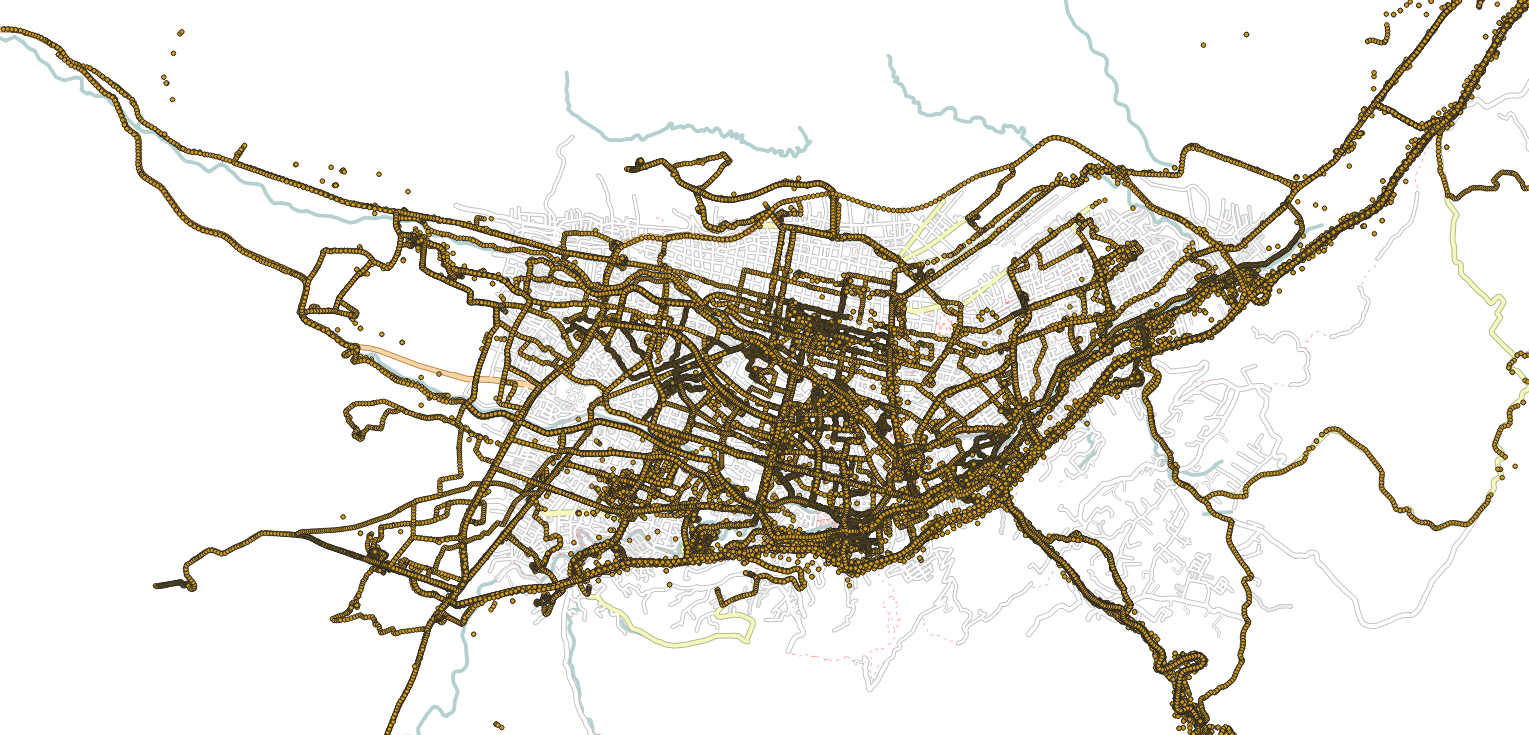
\includegraphics[width=0.9\linewidth]{../paper/images/mapa} \caption{\label{fig2}Sample of collected points for the region of Cuenca, Ecuador.}\label{fig:unnamed-chunk-2}
\end{figure}

\hypertarget{computing-new-attributes}{%
\subsubsection{Computing new
attributes}\label{computing-new-attributes}}

Some additional features must be added to the existing dataset so that
travel behavior can be evaluated.

Let \(p_i\) be the \(i^{th}\) observation in a spatiotemporal dataset
\(P\). Then, the cumulative distance \(D_{a,n}\) for a trajectory
starting at point \(a\) and consisting of the next \(n\) observations is
defined as:

\[ D_{a,n}=\sum_{i=a+1}^{a+n}d_{i, i-1} \] where \(d_{i,j}\) is the
euclidean distance between two observations.

\[ d_{i,j}=((x_i-x_{j})^2+(y_i-y_{j})^2)^{1/2} \]

that is, the sum of distances between proximate points; then, instant
speed at observation \(i^{th}\) is computed by:

\[ s_{i} = \frac{d_{i,i-1}}{t_{i}-t_{i-1}} \] The resulting extended
dataset has the following structure shown in Table \ref{tab2}, after
making the mentioned computations, and then filtering out consecutive
measures taken at the same time stamp (possibly duplicates); also the
very first observation has to be removed in order to avoid division by
zero in the speed calculation. Distances have been transformed to
\emph{km} so that speed unit is \emph{km/h}.

\begin{longtable}[]{@{}
  >{\raggedright\arraybackslash}p{(\columnwidth - 16\tabcolsep) * \real{0.0349}}
  >{\centering\arraybackslash}p{(\columnwidth - 16\tabcolsep) * \real{0.1163}}
  >{\centering\arraybackslash}p{(\columnwidth - 16\tabcolsep) * \real{0.1047}}
  >{\centering\arraybackslash}p{(\columnwidth - 16\tabcolsep) * \real{0.0930}}
  >{\centering\arraybackslash}p{(\columnwidth - 16\tabcolsep) * \real{0.1163}}
  >{\centering\arraybackslash}p{(\columnwidth - 16\tabcolsep) * \real{0.0581}}
  >{\centering\arraybackslash}p{(\columnwidth - 16\tabcolsep) * \real{0.1628}}
  >{\centering\arraybackslash}p{(\columnwidth - 16\tabcolsep) * \real{0.1628}}
  >{\centering\arraybackslash}p{(\columnwidth - 16\tabcolsep) * \real{0.1512}}@{}}
\caption{\label{tab2}Extended dataset with distances and
speeds.}\tabularnewline
\toprule()
\begin{minipage}[b]{\linewidth}\raggedright
\end{minipage} & \begin{minipage}[b]{\linewidth}\centering
x
\end{minipage} & \begin{minipage}[b]{\linewidth}\centering
y
\end{minipage} & \begin{minipage}[b]{\linewidth}\centering
z
\end{minipage} & \begin{minipage}[b]{\linewidth}\centering
t
\end{minipage} & \begin{minipage}[b]{\linewidth}\centering
dow
\end{minipage} & \begin{minipage}[b]{\linewidth}\centering
distance
\end{minipage} & \begin{minipage}[b]{\linewidth}\centering
dt
\end{minipage} & \begin{minipage}[b]{\linewidth}\centering
speed
\end{minipage} \\
\midrule()
\endfirsthead
\toprule()
\begin{minipage}[b]{\linewidth}\raggedright
\end{minipage} & \begin{minipage}[b]{\linewidth}\centering
x
\end{minipage} & \begin{minipage}[b]{\linewidth}\centering
y
\end{minipage} & \begin{minipage}[b]{\linewidth}\centering
z
\end{minipage} & \begin{minipage}[b]{\linewidth}\centering
t
\end{minipage} & \begin{minipage}[b]{\linewidth}\centering
dow
\end{minipage} & \begin{minipage}[b]{\linewidth}\centering
distance
\end{minipage} & \begin{minipage}[b]{\linewidth}\centering
dt
\end{minipage} & \begin{minipage}[b]{\linewidth}\centering
speed
\end{minipage} \\
\midrule()
\endhead
4 & 717002.3 & 9677061 & 2616.9 & 23.30222 & 2 & 0.0008559638 &
0.0030555556 & 0.28013360 \\
6 & 717002.8 & 9677062 & 2616.9 & 23.30444 & 2 & 0.0006438428 &
0.0022222222 & 0.28972928 \\
7 & 717007.8 & 9677053 & 2616.9 & 23.30500 & 2 & 0.0104786529 &
0.0005555556 & 18.86157527 \\
9 & 716998.5 & 9677059 & 2616.9 & 23.33444 & 2 & 0.0112071707 &
0.0294444444 & 0.38062089 \\
11 & 716998.2 & 9677059 & 2616.9 & 23.33500 & 2 & 0.0002436517 &
0.0005555556 & 0.43857315 \\
12 & 717175.5 & 9676911 & 2617.3 & 6.65667 & 3 & 0.2311041122 &
7.3216666667 & 0.03156441 \\
15 & 717228.9 & 9676883 & 2617.3 & 6.65778 & 3 & 0.0602266050 &
0.0011111111 & 54.20394450 \\
16 & 717271.2 & 9676865 & 2617.3 & 6.65861 & 3 & 0.0456284679 &
0.0008333333 & 54.75416151 \\
20 & 717304.9 & 9676851 & 2617.3 & 6.65944 & 3 & 0.0365995628 &
0.0008333333 & 43.91947537 \\
21 & 717338.8 & 9676843 & 2617.3 & 6.66056 & 3 & 0.0350002202 &
0.0011111111 & 31.50019820 \\
\bottomrule()
\end{longtable}

Finally, a last filtering procedure removes observations with extreme
speeds, as values beyond \emph{130km/h} are very improbable (by checking
speed limits within the studied region). These data are often related to
extreme distances between proximate points, which can occur due to GPS
bad measures.

\hypertarget{data-mining}{%
\subsection{Data Mining}\label{data-mining}}

Data traces of each user must be segmented into individual travels
(geometries) so than OD's can be found at the start and end points. In
order to aggregate data into trajectories, an heuristic considering
low-speed hot spots as destinations is now described.

Taken a single day displacements for a single user, the speeds and
distances between proximate points variations that take place when
traveling, staying on destination, changing to a different travel mode
may allow to detect a trip's endpoints. The speed and distance
distributions are shown in Figure \ref{fig3}.

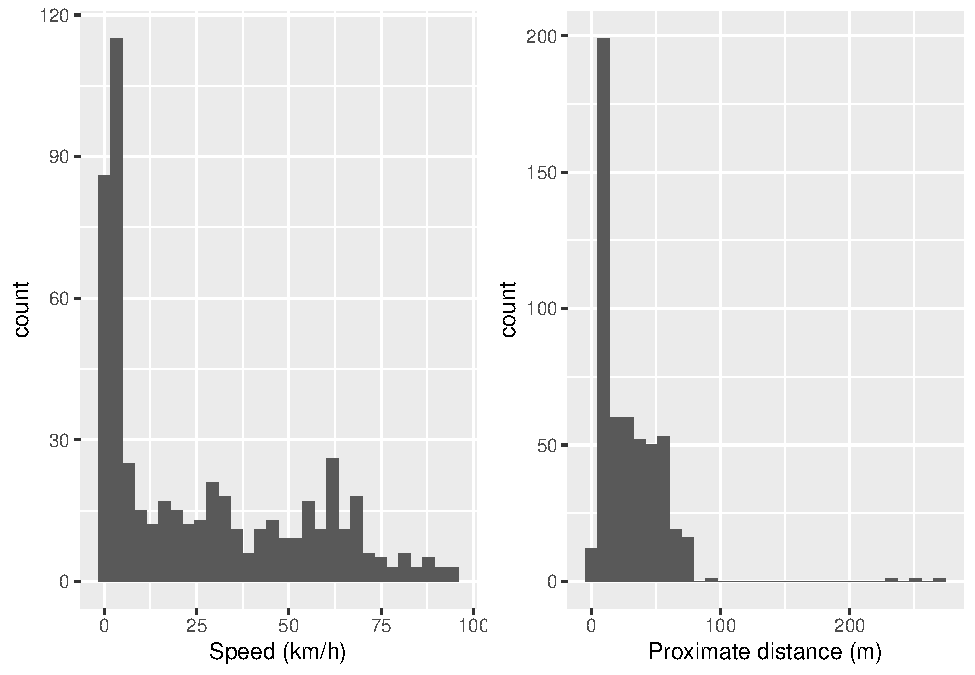
\includegraphics{Elsevier_files/figure-latex/speed-plot-1.pdf} As seen
in the previous figure, most of the speeds and distances are closer to
zero, probably because users spend most of their time walking or staying
in one destination before starting the next trip. The changes in speed
during the day can be seen in Figure \ref{fig4}.

\begin{figure}
\centering
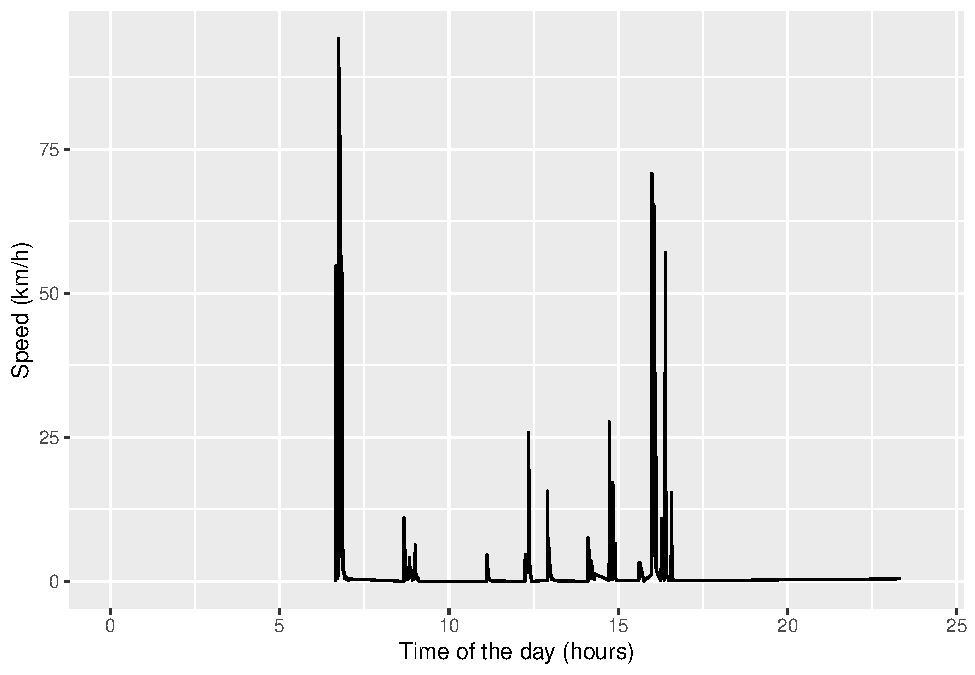
\includegraphics{Elsevier_files/figure-latex/speed-hour-plot-1.pdf}
\caption{\label{fig4}Speed variations along a 24-h single day.}
\end{figure}

This means that, data points can be segmented into individual travels by
detecting those locations when moving at very low speeds (staying
still), with respect to a given speed tolerance \(\epsilon\).

It can be assumed that actual destinations are found in intervals where
users are not moving for a minimum amount of time \(t_{min}\), that is
in the ``valleys'' shown in last figure; in contrast to traffic lights
that will also produce zero speeds but will last only a few seconds. The
following plot allows appreciating points merged into trips (clusters)
for \(\epsilon\)=2km/h and \(t_{min}\)= 10 minutes, see Figure
\ref{fig5}. Increasing \(t_{min}\) will merge nearby trips into larger
ones

\begin{figure}
\centering
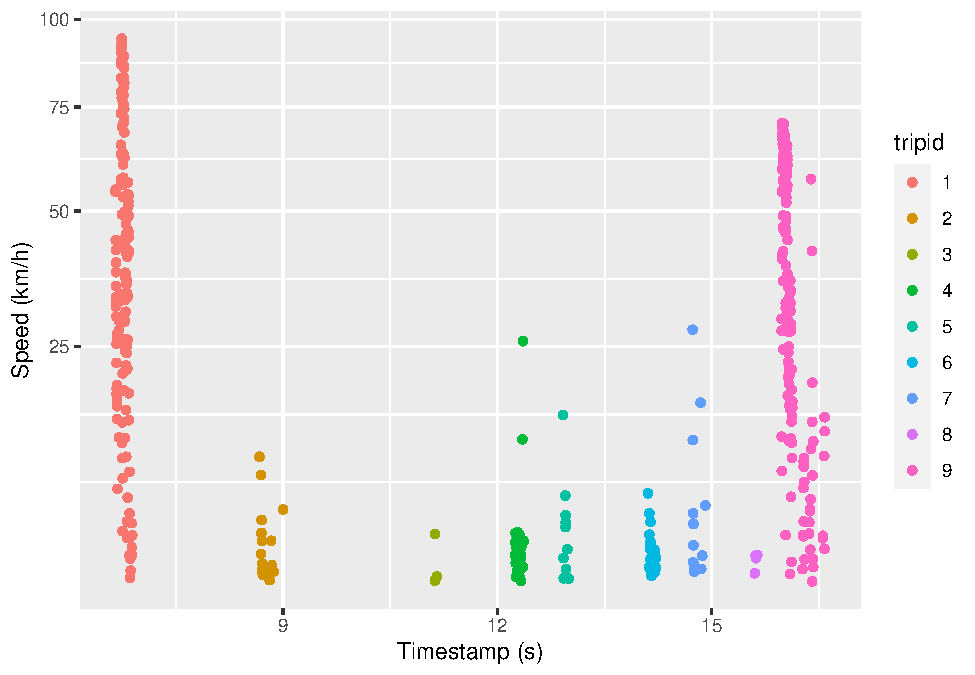
\includegraphics{Elsevier_files/figure-latex/speed-hour2-plot-1.pdf}
\caption{\label{fig5}Speed variations along a single day.}
\end{figure}

At last, the fist (FP) and last (LP) point in each cluster allows
extracting coordinates of the origin and destination, as well as the
departure and arrival times (from the time stamps of these points). The
travel time is simply the difference between the arrival and departure
times; also, the cumulative distance of all points in a cluster
indicates the trip travel distance. The statistics of the extreme points
of each cluster are given in table 3.

\begin{longtable}[]{@{}
  >{\centering\arraybackslash}p{(\columnwidth - 12\tabcolsep) * \real{0.1714}}
  >{\centering\arraybackslash}p{(\columnwidth - 12\tabcolsep) * \real{0.1429}}
  >{\centering\arraybackslash}p{(\columnwidth - 12\tabcolsep) * \real{0.1429}}
  >{\centering\arraybackslash}p{(\columnwidth - 12\tabcolsep) * \real{0.1429}}
  >{\centering\arraybackslash}p{(\columnwidth - 12\tabcolsep) * \real{0.1286}}
  >{\centering\arraybackslash}p{(\columnwidth - 12\tabcolsep) * \real{0.1429}}
  >{\centering\arraybackslash}p{(\columnwidth - 12\tabcolsep) * \real{0.1286}}@{}}
\caption{Extreme points in clusters.}\tabularnewline
\toprule()
\begin{minipage}[b]{\linewidth}\centering
Cluster ID
\end{minipage} & \begin{minipage}[b]{\linewidth}\centering
FP time
\end{minipage} & \begin{minipage}[b]{\linewidth}\centering
LP time
\end{minipage} & \begin{minipage}[b]{\linewidth}\centering
FP x
\end{minipage} & \begin{minipage}[b]{\linewidth}\centering
FP y
\end{minipage} & \begin{minipage}[b]{\linewidth}\centering
LP x
\end{minipage} & \begin{minipage}[b]{\linewidth}\centering
LP y
\end{minipage} \\
\midrule()
\endfirsthead
\toprule()
\begin{minipage}[b]{\linewidth}\centering
Cluster ID
\end{minipage} & \begin{minipage}[b]{\linewidth}\centering
FP time
\end{minipage} & \begin{minipage}[b]{\linewidth}\centering
LP time
\end{minipage} & \begin{minipage}[b]{\linewidth}\centering
FP x
\end{minipage} & \begin{minipage}[b]{\linewidth}\centering
FP y
\end{minipage} & \begin{minipage}[b]{\linewidth}\centering
LP x
\end{minipage} & \begin{minipage}[b]{\linewidth}\centering
LP y
\end{minipage} \\
\midrule()
\endhead
1 & 6.65778 & 6.89056 & 717228.9 & 9676883 & 722215.7 & 9677159 \\
2 & 8.67111 & 9.00083 & 722228.4 & 9677163 & 722206.4 & 9677232 \\
3 & 11.12417 & 11.15306 & 722217.5 & 9677177 & 722219.0 & 9677174 \\
4 & 12.24778 & 12.36639 & 722221.9 & 9677168 & 722402.4 & 9677279 \\
5 & 12.91694 & 12.99778 & 722327.9 & 9677236 & 722198.1 & 9677170 \\
6 & 14.10639 & 14.21889 & 722219.7 & 9677171 & 722319.8 & 9677195 \\
7 & 14.73167 & 14.91028 & 722284.2 & 9677244 & 722319.8 & 9677189 \\
8 & 15.60222 & 15.63500 & 722230.8 & 9677218 & 722186.1 & 9677200 \\
9 & 15.97472 & 16.57806 & 722167.9 & 9676934 & 717010.1 & 9677058 \\
\bottomrule()
\end{longtable}

A glimpse of the aggregate data into individual travels (one per
cluster) is presented in table 4.

\begin{longtable}[]{@{}
  >{\centering\arraybackslash}p{(\columnwidth - 16\tabcolsep) * \real{0.0909}}
  >{\centering\arraybackslash}p{(\columnwidth - 16\tabcolsep) * \real{0.1136}}
  >{\centering\arraybackslash}p{(\columnwidth - 16\tabcolsep) * \real{0.1023}}
  >{\centering\arraybackslash}p{(\columnwidth - 16\tabcolsep) * \real{0.1136}}
  >{\centering\arraybackslash}p{(\columnwidth - 16\tabcolsep) * \real{0.1023}}
  >{\centering\arraybackslash}p{(\columnwidth - 16\tabcolsep) * \real{0.1250}}
  >{\centering\arraybackslash}p{(\columnwidth - 16\tabcolsep) * \real{0.1136}}
  >{\centering\arraybackslash}p{(\columnwidth - 16\tabcolsep) * \real{0.1364}}
  >{\centering\arraybackslash}p{(\columnwidth - 16\tabcolsep) * \real{0.1023}}@{}}
\caption{Sample trips for one single user and day}\tabularnewline
\toprule()
\begin{minipage}[b]{\linewidth}\centering
tripid
\end{minipage} & \begin{minipage}[b]{\linewidth}\centering
ox
\end{minipage} & \begin{minipage}[b]{\linewidth}\centering
oy
\end{minipage} & \begin{minipage}[b]{\linewidth}\centering
dx
\end{minipage} & \begin{minipage}[b]{\linewidth}\centering
dy
\end{minipage} & \begin{minipage}[b]{\linewidth}\centering
departure
\end{minipage} & \begin{minipage}[b]{\linewidth}\centering
arrival
\end{minipage} & \begin{minipage}[b]{\linewidth}\centering
tdistance
\end{minipage} & \begin{minipage}[b]{\linewidth}\centering
ttime
\end{minipage} \\
\midrule()
\endfirsthead
\toprule()
\begin{minipage}[b]{\linewidth}\centering
tripid
\end{minipage} & \begin{minipage}[b]{\linewidth}\centering
ox
\end{minipage} & \begin{minipage}[b]{\linewidth}\centering
oy
\end{minipage} & \begin{minipage}[b]{\linewidth}\centering
dx
\end{minipage} & \begin{minipage}[b]{\linewidth}\centering
dy
\end{minipage} & \begin{minipage}[b]{\linewidth}\centering
departure
\end{minipage} & \begin{minipage}[b]{\linewidth}\centering
arrival
\end{minipage} & \begin{minipage}[b]{\linewidth}\centering
tdistance
\end{minipage} & \begin{minipage}[b]{\linewidth}\centering
ttime
\end{minipage} \\
\midrule()
\endhead
1 & 717228.9 & 9676883 & 722215.7 & 9677159 & 6.65778 & 6.89056 &
6.11272986 & 0.23278 \\
2 & 722228.4 & 9677163 & 722206.4 & 9677232 & 8.67111 & 9.00083 &
0.20374773 & 0.32972 \\
3 & 722217.5 & 9677177 & 722219.0 & 9677174 & 11.12417 & 11.15306 &
0.03148881 & 0.02889 \\
4 & 722221.9 & 9677168 & 722402.4 & 9677279 & 12.24778 & 12.36639 &
0.38327980 & 0.11861 \\
5 & 722327.9 & 9677236 & 722198.1 & 9677170 & 12.91694 & 12.99778 &
0.11186781 & 0.08084 \\
6 & 722219.7 & 9677171 & 722319.8 & 9677195 & 14.10639 & 14.21889 &
0.21750674 & 0.11250 \\
7 & 722284.2 & 9677244 & 722319.8 & 9677189 & 14.73167 & 14.91028 &
0.19505546 & 0.17861 \\
8 & 722230.8 & 9677218 & 722186.1 & 9677200 & 15.60222 & 15.63500 &
0.04114902 & 0.03278 \\
9 & 722167.9 & 9676934 & 717010.1 & 9677058 & 15.97472 & 16.57806 &
6.52144871 & 0.60334 \\
\bottomrule()
\end{longtable}

The resulting segmentation allows OD's to be detected. Their coordinates
are given in the table as attributes ``dx'' and ``dy'' for destinations
locations, and ``ox'' and ``oy'' for the origins. Figure \ref{fig6}
presents on a map at scale 1:25000 the resulting user's destinations (as
red spots). It can be noticed that as locations are repeatedly visited,
some points could be merged into a single destination as possibly they
are short displacements around the same location; this can be done by
density-based clustering techniques; however this is not necessary for
the upcoming analysis.

\begin{figure}
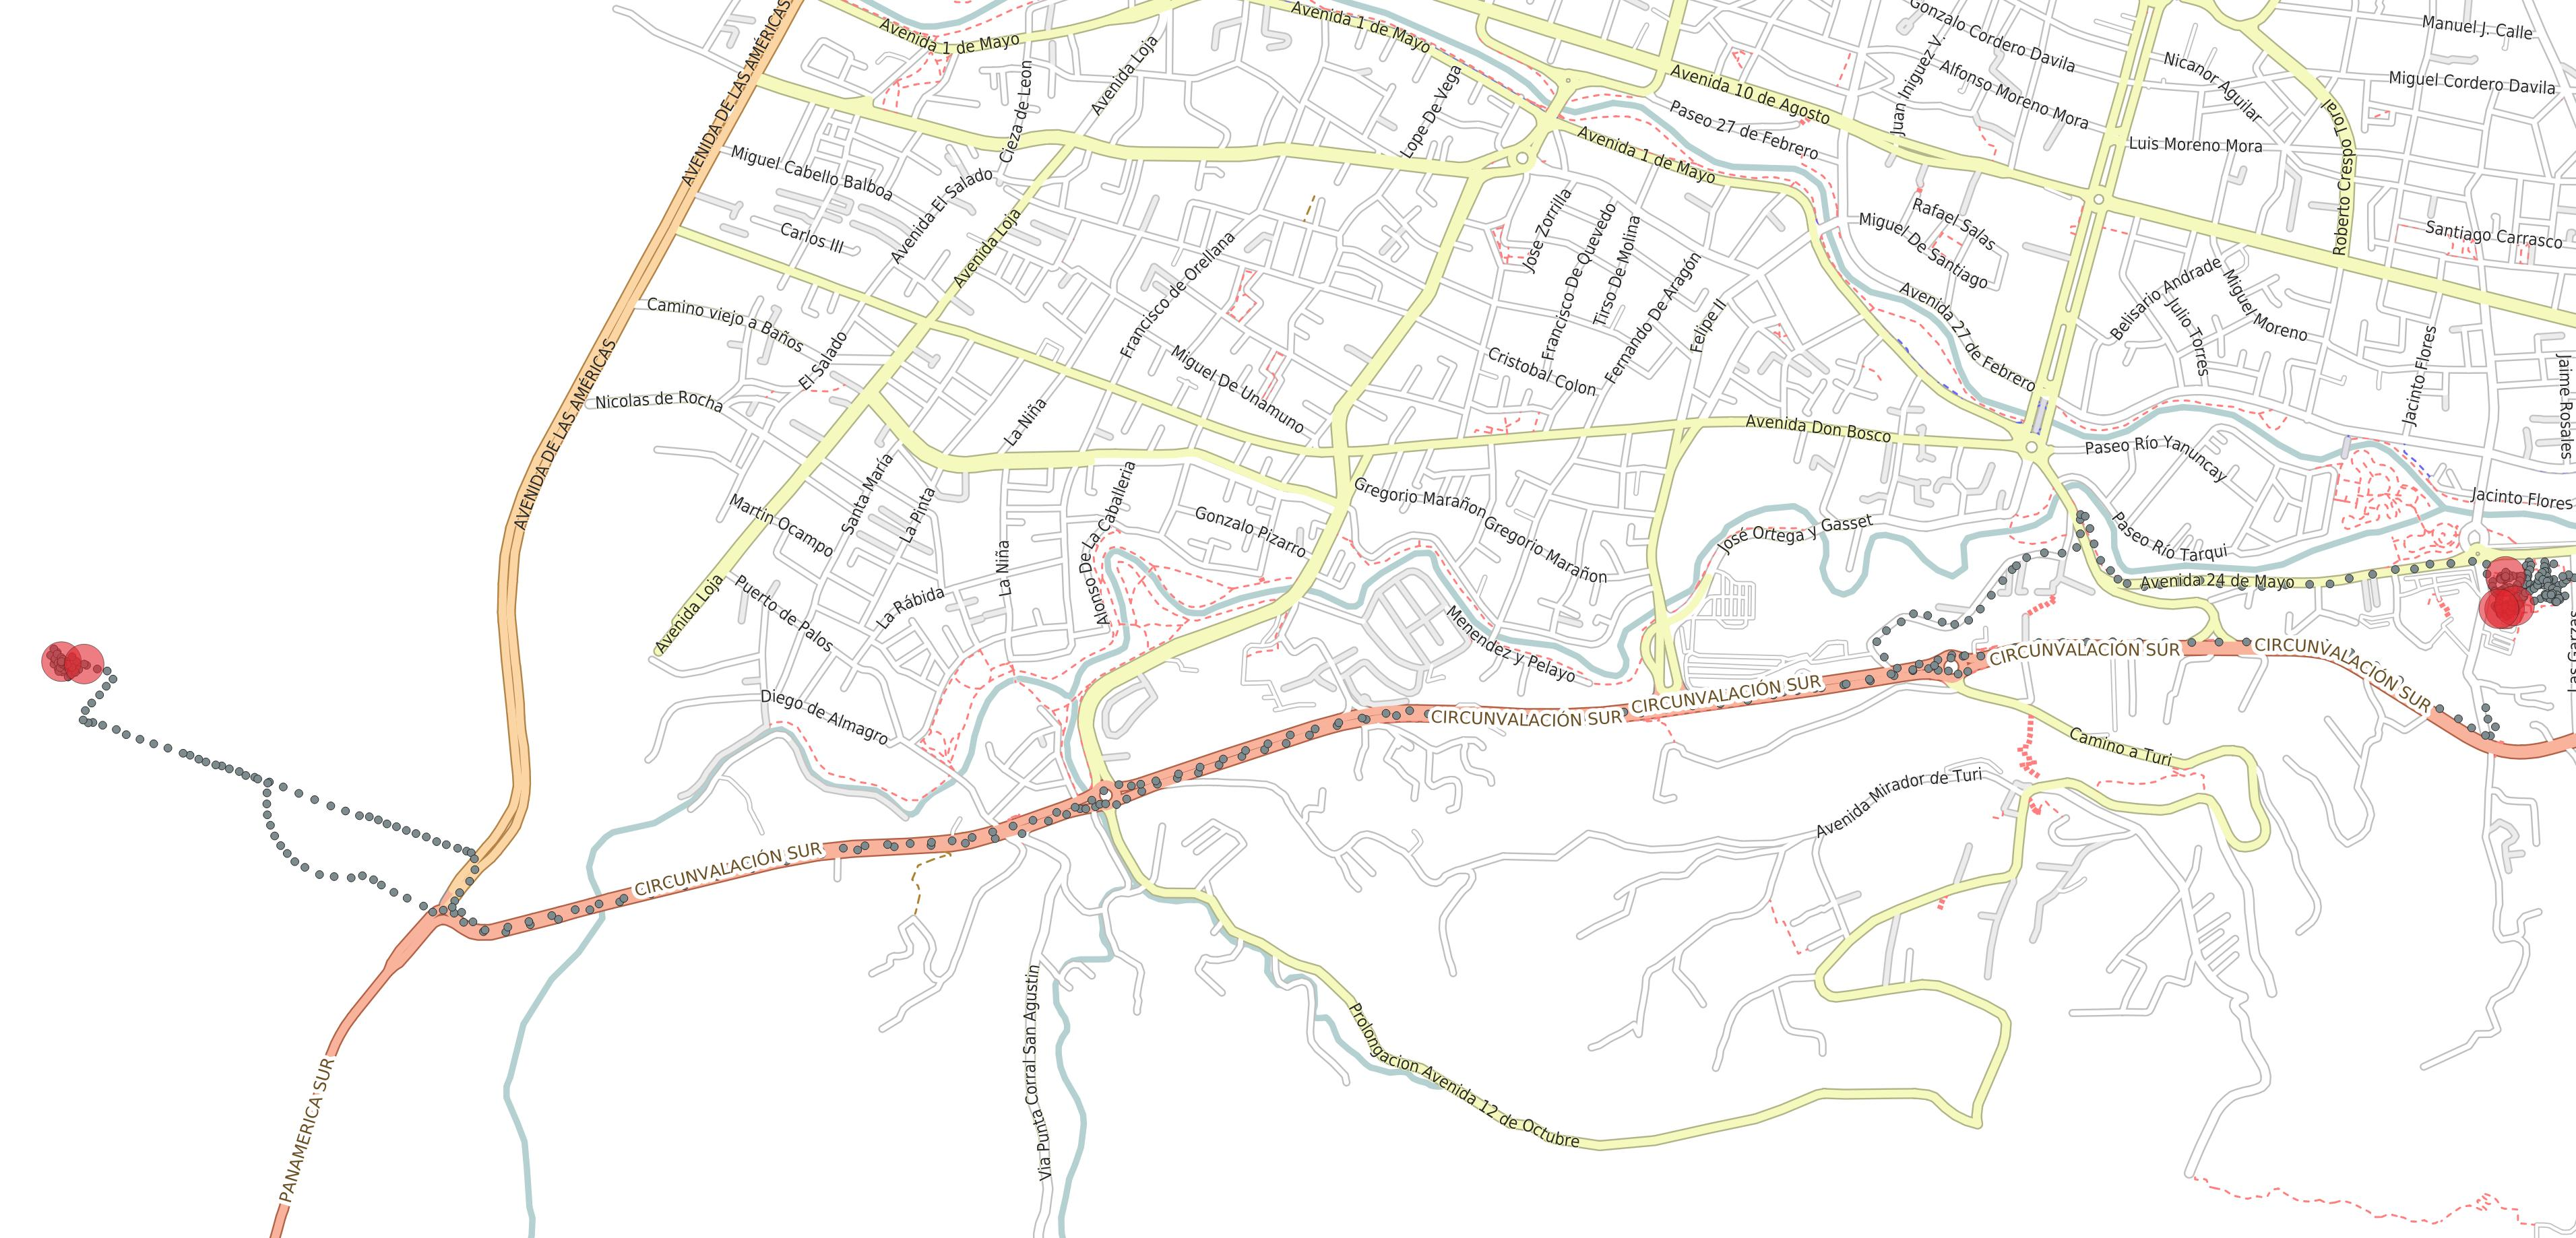
\includegraphics[width=0.9\linewidth]{../paper/images/destinos} \caption{\label{fig6}Sample destinations for one single user and day.}\label{fig:unnamed-chunk-7}
\end{figure}

By applying the algorithm to the full dataset of tracked users,
segmented trajectories exhibit the statistics shown in Figure
\ref{fig7}.

\begin{figure}
\centering
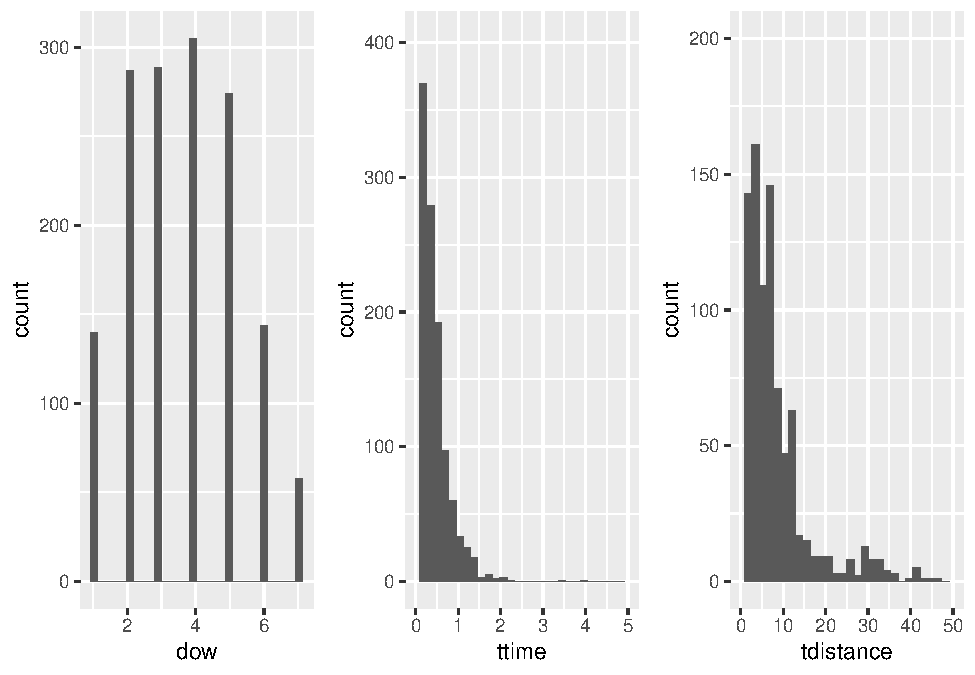
\includegraphics{Elsevier_files/figure-latex/trips-plot-1.pdf}
\caption{\label{fig7}Trip statistics for the full dataset.}
\end{figure}

Then, according to this report, the majority of trips occur on weekdays.
Moreover, they are ``short trips'' below 30 minutes and 10km.

\hypertarget{home-detection}{%
\subsubsection{Home Detection}\label{home-detection}}

After destinations have been detected, another heuristic can be used to
identify a user's home. Another concepts must be first defined.

Let \(T_k\) be a trip displacement identified by \(k\), the following
characteristics are known:

\[T_k=(o_k, d_k, dt_k, at_k, st_k)\]

\begin{itemize}
\item
  \emph{\(o_i\)}, the origin data point with its own coordinates and
  time stamp
\item
  \emph{\(d_i\)}, the destination data point with its own coordinates
  and time stamp
\item
  \emph{\(dt_i\)}, the departure time (time at origin data point)
\item
  \emph{\(at_i\)}, the arrival time (time at destination data point)
\item
  \emph{\(st_i\)}, stay time at destination of this trip
\end{itemize}

\[ st_i =  dt_{i+1} - at_i\]

That is, the stay time is the time spent on destination before the next
trip starts. A first exploratory data analysis must be carried out with
31 users who have voluntarily provided an approximation of the location
of their residence. Some statistics of these trips are presented in
Figure \ref{fig8} (top), where it can be noticed that arrival times of
home trips occur mostly in the evening, in contrast to no-home trips
that do not exhibit a clear pattern as seen in the same figure (bottom).

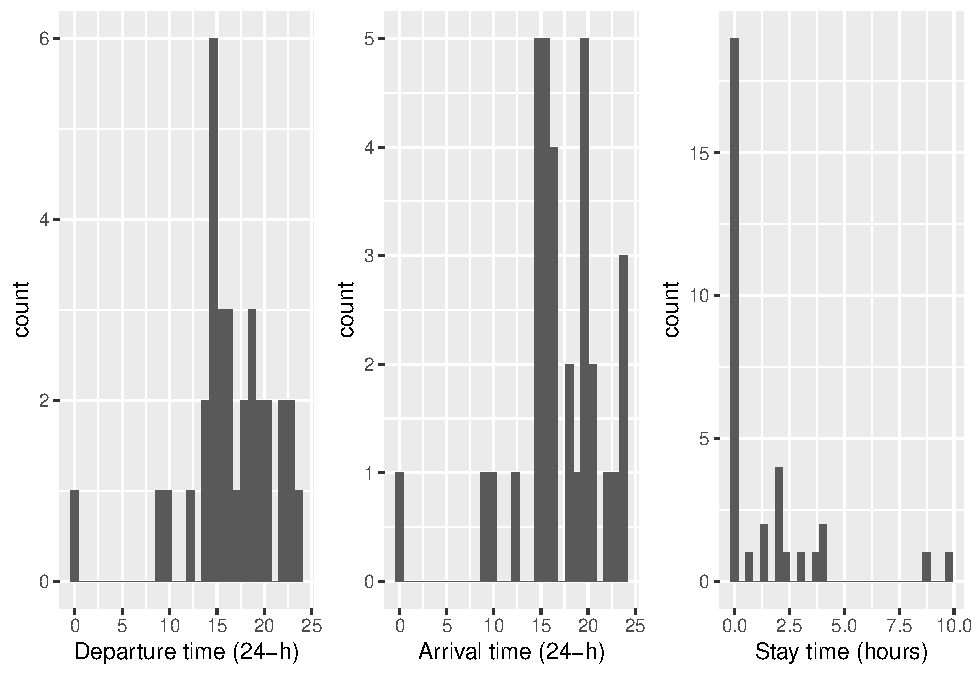
\includegraphics{Elsevier_files/figure-latex/homes-plot-1.pdf}
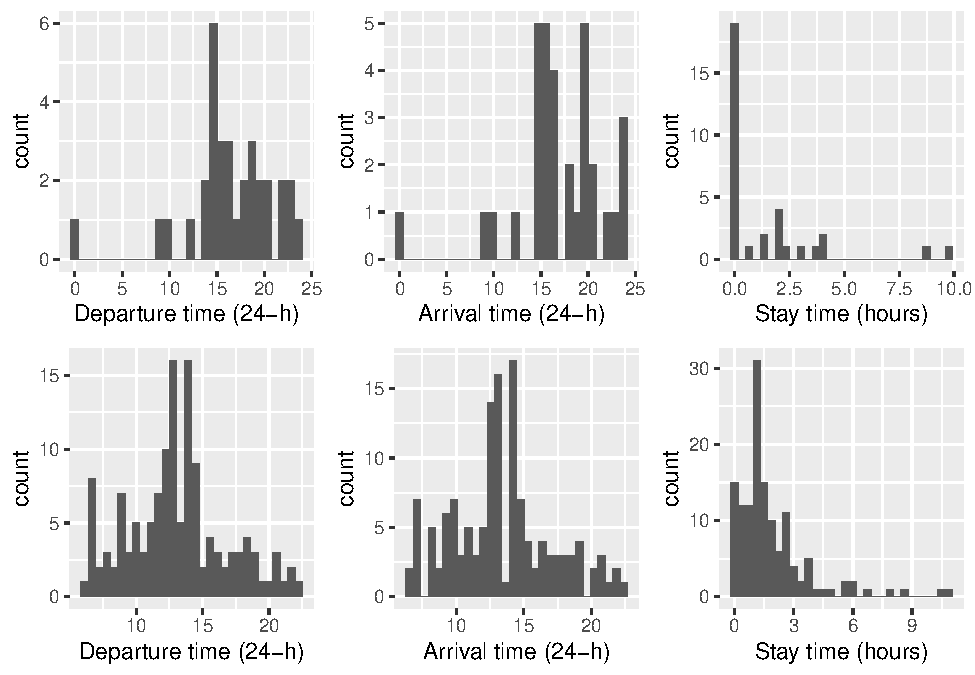
\includegraphics{Elsevier_files/figure-latex/homes-plot-2.pdf}

Taking locations of those destinations found on each last day trip
(avoiding inter-day trips), the results for the same one-user of the
sample used in previous analysis but now for multiple days is shown in
\ref{fig9}.

\begin{figure}
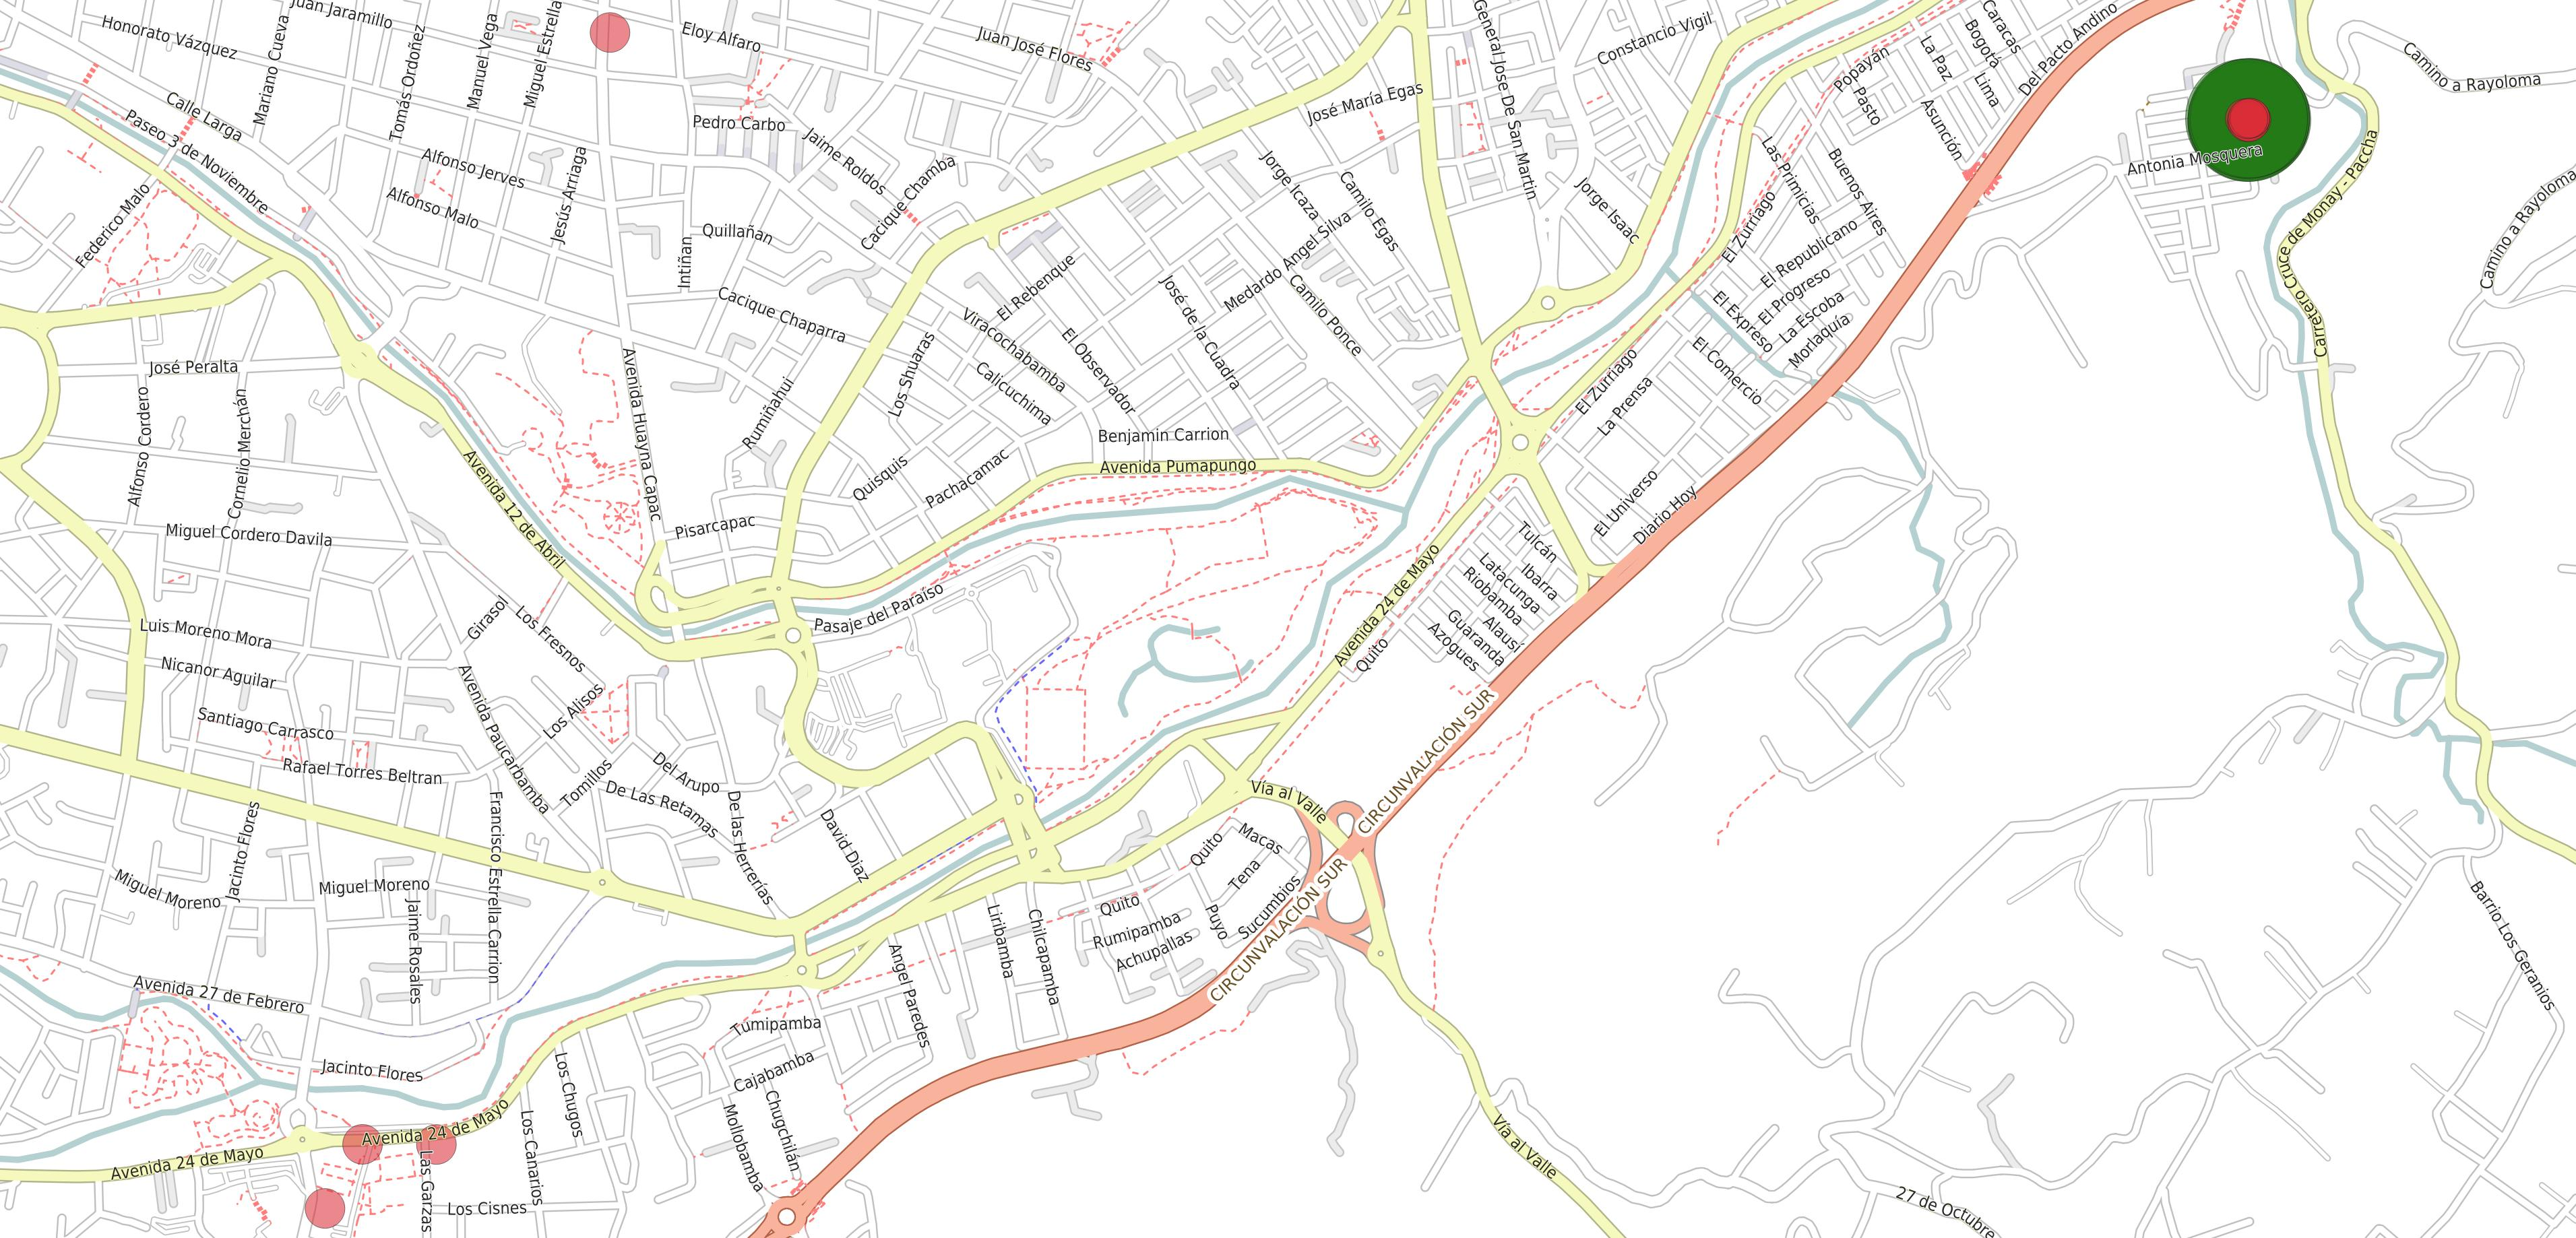
\includegraphics[width=0.9\linewidth]{../paper/images/homes} \caption{\label{fig9}Locations of last day trip destinations for a single user.}\label{fig:unnamed-chunk-10}
\end{figure}

It must be noticed that more than one location could appear as possible
last day trip destination; the most frequent will be labeled as the
``home location''. To find it not only visually, a density based
clustering such as DBSCAN \citep{schubert2017dbscan} must be carried out
on this destination points. The dissimilarity measure of the algorithm
is the euclidean distance to agglomerate single trip destinations into
destinations of interest.

By using a clustering radius of 50 meters with a minimum cluster size of
5 points (which means at least 5 home trips are required to detect it ),
5 different possible candidates were found but only the most frequent
(the biggest cluster) has been assumed to be home as can be seen in the
same Figure \ref{fig9}, where this location has been highlighted as a
green spot.

\begin{figure}
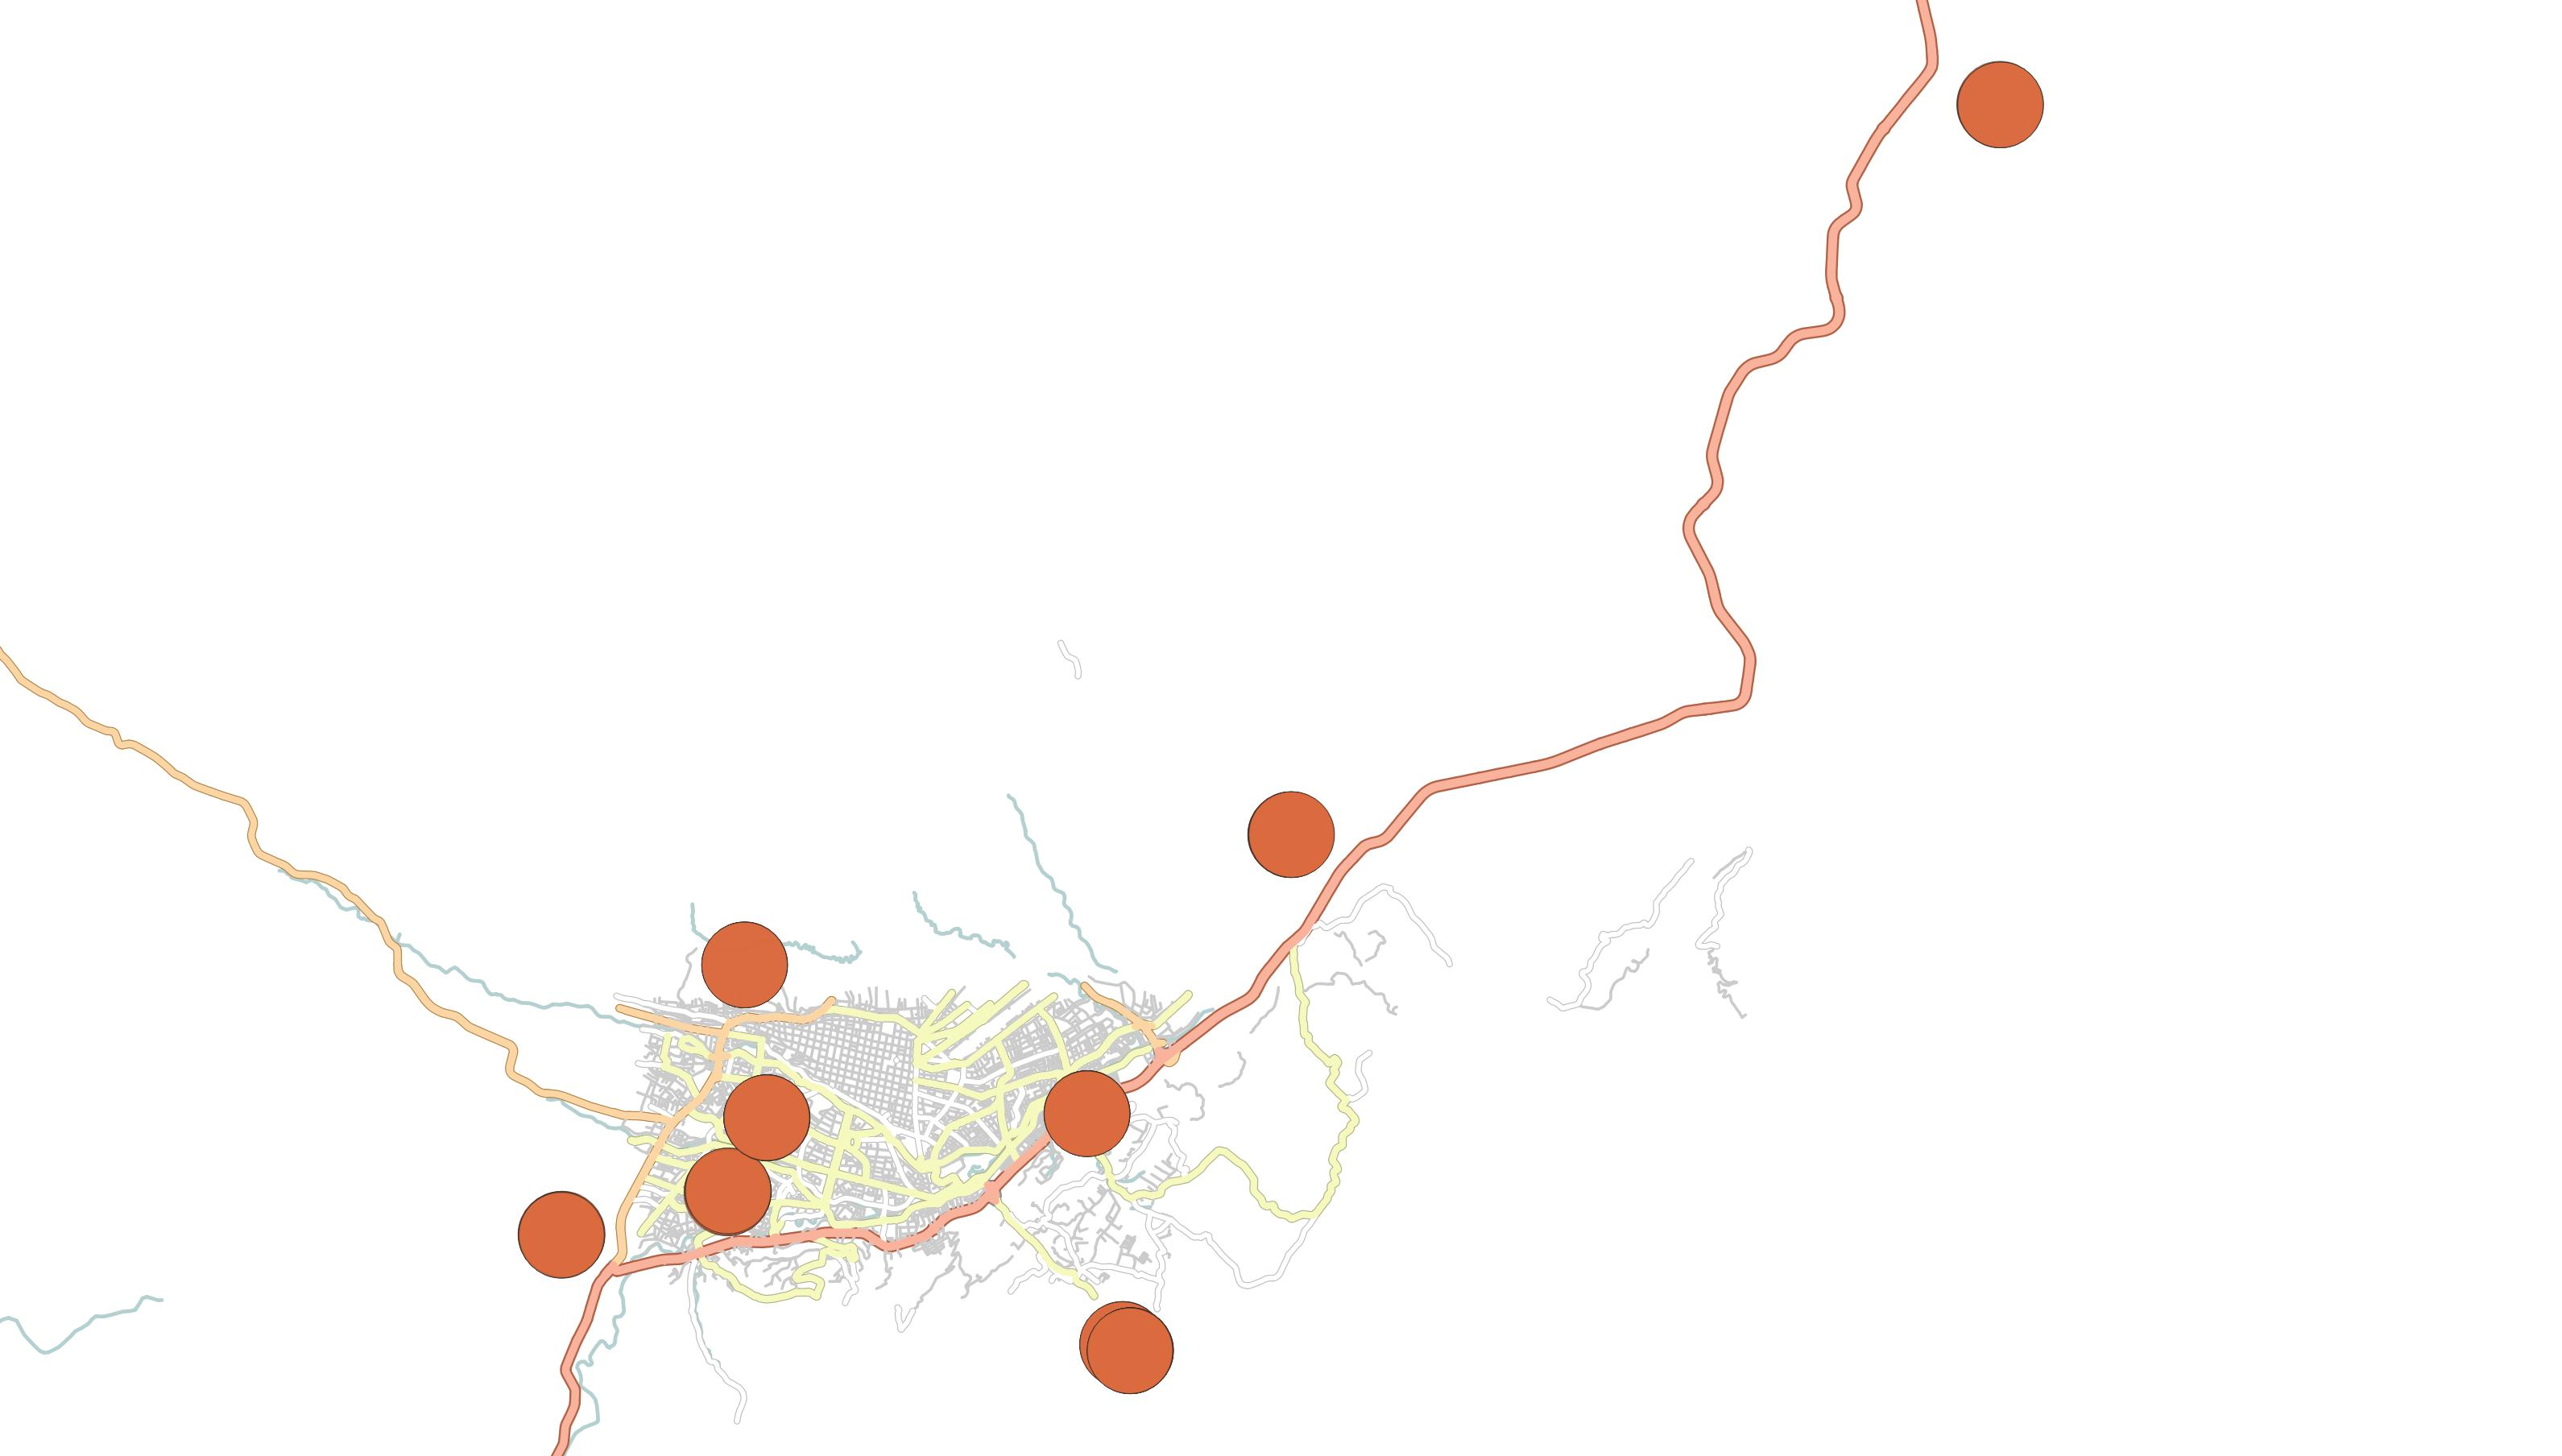
\includegraphics[width=0.9\linewidth]{../paper/images/allhomes} \caption{\label{fig10}Assumed home locations for a sample of users within the studied region of Cuenca, Ecuador.}\label{fig:unnamed-chunk-12}
\end{figure}

\hypertarget{discussion-and-conclussions}{%
\subsection{Discussion and
Conclussions}\label{discussion-and-conclussions}}

This paper states an approach to detect home locations based on data
mining techniques such as clustering, exploratory data analysis and data
segmentation. Home locations have been validated by users who have
voluntarily provided an approximation of the location of their
residence. The heuristic considers the last known destination per day,
so that the more data are collected the more plausible the chance for
the algorithm to capture the correct location. This approach creates
clusters of recurrent destinations, after mobility data is aggregated
into trips by segmentation techniques. It has been shown that one month
of data is sufficient for users to exhibit patterns, which are required
to identify those regions of interest.

The segmentation of data points must be done per user, since OD
detection expects instant speeds to decrease below a reference value per
trip, so that stay time when ``not moving'' reaches a minimum time
threshold. The calibration of these two parameters make trips longer or
shorter, and it could increase the chances to find locations of interest
where the user stays for long periods. As the dataset contains track
points from users, constraining the trips arrival times to an interval
(morning, evening) could detect the college campus as well as home
locations. In the next section some example use cases are provided.

\hypertarget{transport-service-applications}{%
\subsubsection{Transport Service
Applications}\label{transport-service-applications}}

When taking into consideration the home location of several users within
studied area, a list of insights for different applications to provide
transport services arise. A sample of assumed home locations are shown
in \ref{fig10} for our region of interest.

Some possible applications are:

\begin{itemize}
\item
  A dedicated transport service for students at the beginning (end) of
  the day consisting of few bus lines. A current trend is to provide
  college communities with a electric bus service, and this approach
  could led to the design of those bus lines by retrieving the demand
  spatial spots.
\item
  If home locations and the college campus are removed from the trips
  set, then a subset of regions of interest for the students is
  retrieved, providing a list of activities the students perform at
  different times of the day when they are not studying. Private or
  public transport companies could benefit from this information to
  provide services according to the expected departure times.
\item
  At last, carpooling and ride-sharing campaigns could use this
  information to plan groups of students that live nearby, for sharing
  cars and rides to the college campus or other known regions of
  interest.
\end{itemize}

\renewcommand\refname{References}
\bibliography{mybibfile.bib}


\end{document}
